% Chap4-OptimisationSystemeSolaire

\section{Construction d’un système solaire: Un problème d’optimisation multicritère} % (fold)
\label{sec:construction_d_un_systeme_solaire_un_probleme_d_optimisation}
% -----------------------------------
% Rappeler ce qui différencie cette approche des autres issues de la littérature:
%  - Approche couplée système/enveloppe
%  - Optimisation complète systèmes/contrôle/enveloppe

% Aide à la décision nécessite en set de solutions optimales:
%  - Génération d’un jeu de solutions optimales

L’optimisation multi-critère est aujourd’hui largement utilisé dans le bâtiment.
On a par exemple \cite{Armand-Decker2015} qui a développé une méthode d’optimisation pour les
construction bois en utilisant un meta-modèle de bâtiment. Elle utilise un meta-heuristique

à population (Particule Swarm optimization) et évalue les besoins en énergie, le confort des
occupants, la sécurité de l’ouvrage et de l’impact environnemental. \cite{Rivallain2013}
a quand à lui utilisé une méthode approchée (NSGA-II) et une exacte (programmation dynamique)
pour identifier des programmes séquentiels efficaces de réhabilitation énergétique.
Il a ainsi optimisé la combinaison des modifications pour chaque phase mais aussi l’ordre
dans lequel ces améliorations doivent être réalisées afin d’être le plus optimal
possible.
Pour les différentes solutions l’impact environnemental, le confort des occupants en
période estivale, et le coût ont été évaluées.
\itodo{Ajouter des sources vers des exemples d’optimisation de bâtiment}


On a aussi de nombreux exemples d’optimisation de système énergétique.
\itodo{Ajouter des sources vers des exemples d’optimisation de système}

On voit donc que l’optimisation est un outil qui a été largement utilisé dans
le bâtiment comme pour l’amélioration ou l’identification de solutions performantes
pour les systèmes.
L’originalité de ce travail provient principalement du couplage entre le bâtiment
et ses systèmes. La plupart des optimisations de bâtiment évalues les besoins
du bâtiment et considère donc un système de chauffage et de ventilation idéaux.
Dans ces travaux on cherche à optimiser la partie système et son algorithme de
contrôle en même temps que l’enveloppe du bâtiment. On évalue donc plus un besoin
en énergie mais une consommation qui est fonction de la performance des systèmes
envisagées. Les travaux se concentre sur l’évaluation de solutions utilisant fortement
l’énergie solaire comme vecteur énergétique. On cherche donc à couvrir les besoins
de chauffage, d’eau chaude sanitaire (ECS) et d’électricité.
Cette approche permettra d’évaluer le potentiel d’autonomie solaire disponible
pour différentes combinaisons systèmes/enveloppe.
\itodo{Ajouter du bla bla sur l’originalité et les perspectives de ces travaux}

Enfin ces travaux vise à l’élaboration d’un outil d’aide à la décision. Il existe
diverses methodes pour faire de l’aide à la décision comme décrites dans le chapitre
précédent~\autoref{sec:multi_critere}. L’approche choisie est de déterminer un
ensemble de solutions non-dominées dans un premier temps, puis d’utiliser des
outils d’aide à la décision pour réduire le nombre de solution. On se trouve donc
dans une approche par front de Pareto.
\itodo{Ajouter du bla bla sur le choix de l’ordre entre optimisation et aide à la décision}


Dans les sections suivantes nous décrirons dans un premier temps les hypothèses
retenues pour l’étude. Dans un second temps nous décrirons le processus retenu
pour l’outil d’aide à la décision.

\itodo{Reformuler tout ça pour mieux introduire les parties qui suivent}

% section construction_d_un_systeme_solaire_un_probleme_d_optimisation (end)




\section{Cas d’étude: Un système solaire combiné couplée à une maison passive} % (fold)
\label{sec:cas_d_etude_un_systeme_solaire_combine_couplee_a_une_maison_passive}
% -----------------------------------
\subsection{Hypothèses retenues} % (fold)
\label{sub:hypotheses_retenues}
\subsubsection{Description du site étudié} % (fold)
\label{ssub:description_du_site_etudie}
% Description du site étudié:
%  - Climat
%  - Données météos
%  - ...
Afin d’évaluer et d’optimiser la performance d’un système solaire, il est nécessaire
que les conditions extérieures ne soit pas fortement favorable.
Les climats méditerranéens ne sont donc pas des cas d’étude intéressant du fait
de la forte couverture solaire.
À l’opposé le climat de Limoges est assez rude et l’ensoleillement durant la période
hivernale est faible. C’est donc un cas d’étude intéressant.
\itodo{Ajouter une carte pour localiser la ville}
\itodo{Ajouter une description plus complète avec DJU, extrèmes, ...}
\itodo{Refaire complètement ce paragraphe car il fait pitié actuellement}
% subsubsection description_du_site_etudie (end)


\subsubsection{Description de la maison etudiée} % (fold)
\label{ssub:description_de_la_maison_etudiee}
% Description de la maison:
%  - Composition de base
%  - Surface
%  - ...
La maison fait 100\,\si{m^{2}} est est composée de ...
\itodo{Ajouter du bla bla sur la composition de la maison}
% subsubsection description_de_la_maison_etudiee (end)


\subsubsection{Description des scénarios} % (fold)
\label{ssub:description_des_scenarios}
% Descriptions des paramètres fixes:
%  - L’occupation
%  - La température de consigne
%  - Charges internes
%  - ...
Le cas d’étude utilise les scénarios d’une famille moyenne développés au travers de
la création d’un outil pour évaluer l’impact des occupants sur les besoins
énergétiques du bâtiment (\cite{Vorger2014}).
\itodo{Décrire rapidement les travaux d’Éric}

Pour cette étude différents scénarios ont été pris en compte de manière fixe:
\begin{itemize}
    \item Occupation
    \item Charges internes (faibles par rapport à un scénario RT)
    \item Température de consigne
    \item Débits d’extractions d’air
\end{itemize}
\itodo{Décrire les différents scénarios avec des illustrations}

D’autres font partis intégrante de l’optimisation. En effet ils influencent le
fonctionnement du système et donc sa performance. Les scénarios non-fixes sont donc
les suivants:
\begin{itemize}
    \item Occupation
    \item Profil de puisage ECS
    \item Température de consigne solaire
\end{itemize}
\itodo{Décrire les scénarios variables}
% subsubsection description_des_scenarios (end)
% subsection hypotheses_retenues (end)
% section cas_d_etude_un_systeme_solaire_combine_couplee_a_une_maison_passive (end)



\section{Formulation du problème d’optimisation} % (fold)
\label{sec:formulation_du_probleme_d_optimisation}
% -----------------------------------
\subsection{Définition des objectifs et contraintes} % (fold)
\label{sub:definition_des_objectifs_et_contraintes}
\subsubsection{Les objectifs de l’étude} % (fold)
\label{ssub:les_objectifs_de_l_etude}
% Définition des objectifs:
%  - Couverture solaire chauffage
%  - Couverture solaire ECS
%  - Coût de l’installation
%  - Temps de retour sur investissement
Dans cette étude on considère trois fonctions objectifs. On cherche dans un premier
temps à évaluer la performance du système solaire. Pour ce faire on évalue sa
performance sur le chauffage et sur la production d’ECS séparément. Il en a enfin
été noté dans ~\autoref{sec:approche_monozone} que certaines variations impactent
de manière différentes la part de chauffage et d’ECS. Enfin on a vu dans
~\autoref{sub:description_des_systemes} que la production d’ECS reste prioritaire
sur le chauffage, la modification du profil de puisage aura donc un impact différent
sur le chauffage et l’ECS.
\itodo{Il est aussi nécessaire de mettre en valeur l’impact de l’algorithme sur
      les rendements}

Le dernier objectif qui sera pris en compte est l’\textbf{impact économique}. Il
est important de ne pas seulement se focaliser sur la performance du système afin
de filtrer les solutions certes très performantes mais non-réalisable dans les années
proches. Il est ainsi important de rappeler que ces travaux se focalise sur une
technologie innovante mais pouvant être implémentées aujourd’hui.
Ainsi ce facteur bien que discutable du fait de son caractère changeant est indispensable
dans notre étude pour guider la recherche et donner un ordre de prix pour une solution
type.
L’optimisation se portera ainsi sur la maximisation de la couverture solaire pour
(i) le chauffage, (ii) la production d’eau chaude sanitaire, et la minimisation
du coût d’installation et du temps de retour sur investissement.
\itodo{Décrire les différents objectifs retenues avec plus de bla bla}
% subsubsection les_objectifs_de_l_etude (end)


\subsubsection{Les contraintes de l’étude} % (fold)
\label{ssub:les_contraintes_de_l_etude}
% Définition des contraintes:
%  - Surface de toiture à partager (Photovoltaïque)
%  - Équilibre entre production/consommation (Primaire)
Les objectifs sont maintenant clairement définies mais l’étude comporte plusieurs
contraintes qui doivent être prises en compte durant le processus d’optimisation.
La première contrainte est la surface de toiture qui est limitée et doit donc être
partagée entre les panneaux photovoltaïques et thermiques. Comme nous l’avons définie
(~\autoref{sub:description_des_systemes}) le cas d’étude étudié comporte des pans
de toiture avec diverses orientations ce qui complète la première contrainte.
On a donc une double contrainte, à savoir
partager la surface de toiture pour chaque orientation entre les différents capteurs.
Des études ont déjà été réalisées pour évaluer le meilleur ratio entre photovoltaïque
et thermique (\cite{}) mais traite le problème sans tenir compte des combinaisons
entre les équipements, la structure, la régulation, ... Ces travaux permettront donc
d’obtenir plus d’informations sur cet aspect encore aujourd’hui faiblement exploré.
\itodo{Retrouver la publication qui parle de ratio thermique/photovoltaïque}

La seconde contrainte est la place disponible dans la maison pour accueillir les
équipements.
\itodo{Bla bla bla}

Enfin la contrainte principale est sur l’équilibre entre production et consommation
d’énergie primaire. En effet l’approche MEPOS ou encore NZEB définit comme requit
pour une maison passive d’avoir un équilibre entre production et consommation.
On a donc ici une contrainte forte au niveau énergétique.
\itodo{Bla bla bla}
\itodo{Décrire les contraintes et la méthode utilisée pour les traiter}
% subsubsection les_contraintes_de_l_etude (end)
% subsection definition_des_objectifs_et_contraintes (end)
% section formulation_du_probleme_d_optimisation (end)


\subsection{Choix des variables de décision} % (fold)
\label{sub:choix_des_variables_de_decision}
% Choix des variables de décisions:
%  - Propre au bâtiment
%  - Propre au système
%  - Propre au contrôle
Dans cette partie sera décrit les différentes variables qui ont été sélectionnées
en amont du **screening**.
\itodo{Décrire l’ensemble des variables considérées en amont de l’étude de sensibilité
      classée par groupe, système, contrôle, enveloppe, scénarios}
% Définir chaque variable:
%  - Type
%  - Plage de variation
%  - Unité
%  - Description
\itodo{Dresser une liste des caractéristiques de chaque critère}
\itodo{Faire apparaître clairement (graphiquement) l’impact de chaque variables
      sur les différents objectifs peut être pas à mettre ici mais plus dans
      ~\autoref{sub:reduction_de_la_cardinalite_par_screening}}
% subsection choix_des_variables_de_decision (end)




\section{Méthode retenue pour le dimensionnement du système} % (fold)
\label{sec:methode_retenue_pour_le_dimensionnement_du_systeme}
% -----------------------------------
Comme nous l’avons vu précédemment, il existe de nombreux meta-heuristiques dans
la littérature. Cependant il n’existe pas à la connaissance de l’auteur de méthode
pour sélectionner un algorithme qui sera le plus performant pour un problème donnée.
Ce principe a été formalisé par \cite{Wolpert199767} \itodo{Pas encore lu ...}. Il démontre qu’il
n’y a aucunes \emph{à priori} différences entre les algorithmes. Les critères
permettant de sélectionner un meta-heuristique sont donc à caractère subjectif.
Un des arguments pertinent qui peut être mis en avant est le nombre de paramètres
nécessaires pour le réglage de l’algorithme. En effet sur ce point les algorithmes
sont très différents, certains demandant de nombreux paramètres à configurer
\itodo{Citer des exemple de algo génétique, réseaux de neuronnes, ...} contrairement
à d’autres \itodo{Citer des exemples de PSO, ABC, ...}. Un autre critère pertinent
est la robustesse des algorithmes. On entend par \emph{robuste} la capacité des algorithmes
à converger pour différentes valeurs de paramètre. Par exemple le meta-heuristique PSO
peut être considérée comme robuste \itodo{Mettre des sources} car la solution n’est
pas fortement influencée par le choix de la configuration.
À l’opposée des approches par réseau de neurones \itodo{Mettre des sources} sont
très sensibles, et la variation d’un paramètre peut donner une solution complètement
différente (pour le meilleur et le pire).
Afin de pallier à ces problème, des outils existent pour paramétrer ces meta-heuristique.
C’est particulièrement vrai dans le cas d’optimisation mono-critère mais commence
aussi à émerger pour des problème plus complexe. \cite{Lopez-Ibanez2012861}
présente un framework pour faire de l’optimisation multi-critères en utilisant
différents algorithmes de colonies de fourmis (MOACO). Il propose aussi un outil
pour configurer automatiquement les paramètres du meta-heuristique en utilisant un jeu de solution
d’entrainement. Pour ce faire les auteurs ont adapté l’algorithme \emph{F-Race} (\cite{Lopez-Ibanez2011})
au problème multi-critère pour différentes (\cite{Birattari2010311,Zitzler2003117}). Les auteurs montrent
alors que les configurations trouvées automatiquement sont meilleures que celles
de la littérature pour différents type de problèmes. Cette approche permet alors
de se passer de l’étape de configuration manuelle et pourrait si généralisée/généralisable
permettre au meta-heuristique très dépendant de ces paramètres d’être plus simples
à utiliser.
\itodo{Vu le nombre de choses à dire, faire le tri entre ce qui va ici et ce qui
      va dans le chapitre précédent. . .}
Au vu des remarques précédentes le meta-heuristique choisi est basé sur le
comportement des abeilles, une approche assez récente \itodo{Mettre citation}.Il est
robuste \itodo{Ben ouais citation} et comporte peu de paramètre à tuner. Enfin il
a montré sa capacité à sortir des minimums locaux \itodo{citation toujours citation}.
La partie suivante présente ce générateur de solution de manière plus détaillée.
\itodo{Faire un comparatif des solutions existantes convergence/répartition/vitesse
      et mettre en exergue la lenteur de mes simulations ...}
% subsection methode_retenue_pour_le_dimensionnement_du_systeme (end)


\subsection{Optimisation par essaim d’abeilles: un meta-heuristique à population} % (fold)
\label{sub:optimisation_par_essaim_d_abeilles_un_meta_heuristique_a_population}
% Description du Meta-heuristique choisi:
%  - Origine de l’algorithme (inspiration des abeilles):
% Décrire l’origine de cet algorithme. Décrire les recherches qui ont été faites sur
% les abeilles et ensuite les conclusions tirées par l’inventeur pour formuler ce
% meta-heuristique.
% Les sources suivantes non pas encore été lues: \cite{Camazine1991547}, \cite{Seeley1996}
% mais traitent du comportement des abeilles.
%  - Formulation théorique:
%     + Description des différentes étape de résolution de la méthode:
%       Détails pour onlookers, employed, scout, ...
%       Détails pour les paramètres nécessaires au fonctionnement de l’heuristique.
%     + Description de la mise à jour de la position d’une source:
%       Dans le cas de variables continues la formulation de base est applicable et sera
%       donc conservée. Dans le cas de variables discrètes on utilisera une méthode alternative
%       développée dans `10.1177/0021998308097681` et `tel-01234197, version 1`.

L’intelligence artificielle se traduit par la construction de programmes informatiques
pour la réalisation de tâches demandant une démarche critique, et de l’apprentissage. La
notion a été inventé par John McCarthy et Marvin Lee Minsky et ne cesse de s’améliorer
dans de nombreux domaines comme le déplacement organisé de groupe important d’animaux (humains, oiseaux, poissons, ...)
ou encore l’apprentissage et la réflexion (\cite{Hsu199970,Silver2016484}).
Une des branches de l’intelligence artificielle s’intéresse particulièrement au comportement
du monde animal. Dans notre cas on s’intéresse à la branche de l’intelligence des
essaims (Swarm Intelligence). \cite{Bonabeau1999} a définit quatre caractéristiques
définissant l’organisation dans ces essaims:
\begin{description}
    \item \emph{positive feedback}, se traduisant par le renforcement de chemins ou le recrutement d’individus suite à un constat
          d’un des individus
    \item \emph{negative feedback}, permettant de stabiliser la structure évitant la saturation du au positive feedback facteur
    \item \emph{fluctuations ou amplification}, faisant émerger des solutions nouvelles (facteur aléatoire)
    \item \emph{multiple interactions}, pouvant se traduire par le partage d’informations entre les individus de la population
\end{description}
Les algorithmes les plus connues étant inspirées des oiseaux (Particule Swarm Intelligence),
des fourmis (Ant Colony), ou encore des abeilles qui a été choisi pour les raisons explicité ci-avant.
Il existe plusieurs approches d’algorithmes d’essaims d’abeilles. Certaines sont basées
sur le comportement des butineuses faisant intervenir la fameuse danse des abeilles pour partager
les informations sur la qualité d’une source aux autres abeilles. D’autres s’inspirent de la
reproduction des reines ou encore du mariage.
Parmi les plus utilisés on peut citer le mariage entre abeilles introduit par \cite{Abbass20011}, l’algorithme VirtualBee
créé à l’origine pour l’optimisation de fonction numérique \cite{Yang2005317}, l’algorithme Bee Colony Optimization (BCO)
\cite{Lucic2001441} pour l’optimisation de problèmes combinatoire. Enfin on peut citer les
algorithmes BeeHive proposé par \cite{Wedde200483} et les algorithmes Artificial Bee Colony (ABC) introduit par
\cite{Karaboga2005}. ABC simule le comportement des butineuses pour la recherche de sources prometteuses.
Comme le montre l’état de l’art de \cite{Karaboga201221} il est l’algorithme le plus
utilisé pour la résolution de problèmes d’optimisation et peut être appliqué à toute sorte de problème: continues,
combinatoires, mono et multi-objectifs, contraints, ou encore pour faire du clustering.

À l’origine pensé pour résoudre des problèmes continues il a été adapté pour traiter des problèmes
d’optimisation binaire \cite{Kashan2012342}, combinatoire \cite{Karaboga20113021}, et pour des cas multi-critères
\cite{Akbari201239,Omkar2011489}.
Ce méta-heuristique a été utilisé pour résoudre des problèmes de tout type, dont l’entrainement de réseaux de
neurones (\cite{Karaboga2007}), le génie électrique/mécanique/civil (\cite{Rao2009887}), ou encore le clustering (\cite{Zhang20104761}).
On retrouve aussi cet algorithme dans l’optimisation de système de chauffage (\cite{Atashkari2011}) ou dans des problèmes avec
contrainte (\cite{Tsai201480,Karaboga20113021}).
Malgré son jeune âge la littérature sur les colonies d’abeilles augmente exponentiellement et continue de se diversifier
pour mieux répondre aux différents types de problèmes d’optimisations.
\itodo{Ajouter un graphique montrant l’attrait pour ces techniques \cite{Karaboga201221}}


\itodo{Décrire l’algorithme}
Dans la partie qui suit l’approche retenue pour ces travaux, l’algorithme ABC, est détaillée.
Dans la nature les abeilles communiquent entres elles pour découvrir et récupérer le plus
de nectar possible. Leur comportement est défini par principalement 3 composants:
\begin{description}
    \item La source de nourriture: Elle est caractériser par sa quantité, proximité, et accessibilité.
    \item Les butineuses (employed foragers): Elles évaluent la qualité des sources explorées et ramènent cette information
          au reste des abeilles dit réceptrices (unemployed foragers). L’information de chaque source est transmisse
          grâce à une danse. Celle-ci permettant de donner la qualité et la direction d’une source.
    \item Les réceptrices (unemployed foragers) se décomposent en deux groupes:
    \begin{itemize}
        \item Les spectatrices (onlookers) qui utilisent l’information des butineuses pour sélectionner une source à exploiter.
              Plus la source est de qualité plus grande est la probabilité qu’une spectatrice la choisisse.
        \item Les éclaireuses (scouts) qui explorent aléatoirement les environs, à la recherche d’une nouvelle source. On estime à
        5-10\,\% la quantité de d’éclaireurs dans un essaim \cite{Seeley1996}
    \end{itemize}
\end{description}
\etodo{Ajouter les formulations mathématique et algorithmiques}
\ftodo{Ajouter une description graphique de l’algorithme ou un flowchart}

\itodo{Description de l’algorithme au niveau global avec des renvois vers chaque phase.
      Faire un table avec une description des différentes phases et l’algorithme global au-dessus ?}
L’algorithme ABC peut ainsi se traduire par les différentes étapes suivantes:

\itodo{Décrire les caractérisation qui ont été évalué (taille population, nombre de cycle, convergence, ...): }
L’algorithme étant encore jeune de nombreuses améliorations et/ou modifications on été ajouté au cours des dernières années.
\cite{Aderhold2010283} a évalué l’impact de la taille de la population et propose une nouvelle méthode
pour mettre à jour la position des sources. Certaines améliorations s’inspirent du PSO en tenant compte d’un facteur
d’inertie ou de la meilleure solution globale (\cite{Lei2010,Zou20109}).
D’autres s’inspirent de algorithmes évolutionnaires et génétiques (\cite{Bi2011174,Zhao2010558}). Il a aussi été développé
de nombreuses approches hybrides dont \cite{Pulikanti2009196} utilisant un heuristique.


\itodo{Ajouter une description des approches pour améliorer ABC à cause des problème d’exploitation (Sharma2012213 p.217 pour blabla)}
Un meta-heuristique se compose de deux étapes principales, l’exploration et l’exploitation.
L’exploration est mesurée par la capacité à explorer l’espace de solution à la recherche
des zones prometteuse pour un optimum.
Cependant une fois ces zones trouvées, une autre approche est nécessaire: l’exploitation.
L’exploitation consiste à l’aide de l’information disponible sur le voisinage et sur la solution actuelle
de l’améliorer et donc de converger vers un optimum.
Afin d’éviter de tomber dans un optimum local ou bien de converger très lentement, un équilibre entre exploration et
exploitation est nécessaire.
Dans notre cas l’algorithme ABC est reconnue pour être bon en exploration mais faible en exploitation (\cite{Karaboga2009108,Zhu20103166,Karaboga201221}).
En effet le paramètre $limit$ et les éclaireuses permettent d’éviter de se coincer dans un optimum local, cependant
l’essaim n’utilise pas autant d’informations pour la recherche locale que par exemple le PSO. Il en résulte une converge
plus lente vers l’optimum. Pour remédier à ce problème de nombreuses approches ont été envisagées.
\cite{Zhu20103166,} ajoute la prise en compte de
la meilleure solution actuelle dans l’équation de mise à jour
Il nomme le nouvel algorithme Gbest Artificial Bee Colony (GABC) et la nouvelle formulation
de la mise à jour\emtodo{Ajoute mise à jour de l’équation} est décrite ci-dessous:
Pour contrôler l’importance de la meilleure solution actuelle un coefficient est tiré aléatoirement
selon une distribution uniforme ($\psi_{ij}$). La borne maximale $C$ de la distribution est définie par l’utilisateur et
l’augmenter correspond à augmenter l’importance de la meilleure solution actuelle.
\cite{Li2012320} propose une autre variante en ajoutant une inertie, une accélération, et l’influence de la meilleure actuelle et
le nomme Improved Artificial Bee Colony (I-ABC).
Il propose aussi une seconde variante faisant évoluer 3 essaims avec 3 algorithmes différents (PS-ABC). Il est cependant
important de rester prudent sur l’interprétation des résultats, particulièrement sur la variante PS-ABC. En effet comme
le décrit \cite{Mernik2015115}, les algorithmes doivent être comparés suivant le nombre d’évaluations de la/les fonctions
objectifs et non par rapport au nombre d’itérations. En effet la variante PS-ABC ici utilise 3 populations et réalise donc
en moyenne 6 fois plus d’évaluation de fonction par itération que l’approche standard.
On peut aussi citer \cite{Aderhold2010283,Karaboga2014227} qui ajoutent respectivement la distance euclidienne pour la sélection
de solution optimales proches, et la différenciation entre butineuses et spectatrices pour la mise à jour des sources.

Plusieurs approches ont aussi été envisagées pour les problèmes multi-objectifs. On a par exemple l’approche MO-ABC, VABC, MHABC-CMO
\cite{Hedayatzadeh2010, Akbari201239} adapte l’algorithme ABC pour résoudre des problèmes multi-objectifs. Ils proposent
principalement deux modifications. La première est l’utilisation de l’$\varepsilon$-dominance \mtodo{Ajouter un lien vers l’explication}
pour la gestion de l’archive assurant ainsi la diversité des solutions. La seconde modifie la mise à jour des sources en
exploitant la population et les solutions de l’archive.
\cite{Zhang20121} introduit une approche basée sur plusieurs essaims se partageant les informations et une sélection
des solutions du front de Pareto par crowding distance. Le papier propose une comparaison avec d’autres approches sur un ensemble de
problèmes multi-objectif avec contraintes.
Enfin on peut aussi noter l’approche de \cite{Omkar2011489} qui cherche à optimiser chaque objectifs séparément et nomme l’approche
Vector Evaluated Artificial Bee Colony (VEABC). Chaque individus d’un
essaim sont mis à jour en utilisant les individus des autres essaims. C’est cette collaboration qui permet à l’algorithme
de trouver l’espace de compromis.


\itodo{Décrire les approches pour tacler les problèmes avec contraintes}


\itodo{Décrire Lévy Flight et applications}
Nous avons vu que le maintien de l’équilibre entre exploitation et exploration est un
critère fondamental pour la formulation d’un meta-heuristique performant. Cependant il y a un caractère
inhérent à chaque méta-heuristique dont nous n’avons pas parlé: l’aléatoire.
Les méta-heuristiques sont alors dits stochastiques; en plus de l’échange d’informations entre les individus, l’aléatoire
à un rôle très important.
Les méthodes approchées ont en effet été développées afin de répondre aux besoins d’optimisation sur des
problèmes dont la connaissance à-priori est insuffisante pour formuler le problème sous une forme classique.
Certains auteurs ont alors cherché à améliorer les algorithmes en modifiant la loi de
distribution utilisée, s’inspirant encore une fois du monde du vivant.




Dans un premier temps, il est important de définir le terme de marche aléatoire inhérent
à beaucoup de méthodes approchées.
Une marche aléatoire (\cite{Yang201445}) peut être définie comme une succession de pas
aléatoire dont chaque état ne dépend que de l’état précédent. Si on note $S_{N}$
la somme des pas aléatoires consécutifs $X_{i}$ alors $S_{N}$ est une marche aléatoire:
\begin{equation}\label{eq:marche_aleatoire}
    \begin{split}
        S_{N} &= \sum_{i=1}^{N} X_{i} = X_{1} + ... + X_{N}\\
              &= S_{N-1} + X_{N}
    \end{split}
\end{equation}
Il est alors clair d’après la forme récursive de \eqref{eq:marche_aleatoire} que l’état suivant
ne dépend que de l’état précédent.


La longueur du pas peut varier en fonction de la distribution de probabilité à laquelle il est associé.
Les plus utilisées dans les méta-heuristiques étant les loi uniformes, comme par exemple dans les algorithmes PSO ou ABC.
Il existe de nombreuses autres distributions, poisson, normale (ou gaussienne), ou encore de Lévy.
\ftodo{Densité de probabilité des loi existantes}

C’est cette dernière qui nous intéresse plus particulièrement pour une application en méta-heuristique.
Il a en effet été observé chez diverses espèces comme les atèles (singes), les albatros,
ou encore la famille des Tephritidae (petites mouches) un comportement respectant
une marche aléatoire connu sous le nom de Lévy Flight.\mtodo{Citations de Sharma2012213 et Yang201445}
Cette marche aléatoire est une marche aléatoire utilisant une distribution de Lévy pour
déterminer la longueur du pas aléatoirement.
La distribution de Lévy de son auteur Paul Lévy est une distribution à queue lourde, indiquant que son comportement
éloignée de la zone centrale de la distribution n’est pas exponentiellement bornée.
La loi de Lévy dépend de deux paramètres: $\nu > 0$ qui est le pas minimum et $\gamma > 0$ qui est le
facteur d’échelle.
La densité de probabilités peut ainsi s’écrire sous la forme analytique simplifiée suivante (\cite{Yang201445}):
\begin{align}\label{eq:dens_levy}
    L(s, \gamma, \mu) = \begin{cases}
                            \sqrt{\frac{\gamma}{2\pi}} \exp\left[-\frac{\gamma}{2(s-\mu)}\right] \frac{1}{(s-\mu)^{\nicefrac{3}{2}}} &\ 0 < \mu < s < \infty \\
                            0                                                                                                        &\ sinon
                        \end{cases}
\end{align}
La distribution est le plus souvent exprimée sous la forme d’une transformée de Fourier:
\begin{equation}\label{eq:fourier_levy}
    \mathcal{F}(k) = \exp(-\alpha|k|^{\beta}) \qquad  0 < \beta \leq 2
\end{equation}
Il existe des cas spéciaux où la transformée inverse de Fourier correspond à une distribution
normale ($\beta = 2$), ou une distribution de Gauchy ($\beta = 1$).

La forme analytique de la \emph{distribution de Lévy stable et symétrique} (symmetrical Lévy stable distribution with index $\beta$) peut
s’exprimer sous la forme suivante (\cite{Gutowski2001}):
\begin{equation}\label{eq:dist_levy}
    L(s) = \frac{1}{\pi} \int_{0}^{\infty} \cos(k s)\exp(-\alpha k^{\beta}) dk \qquad  0 < \beta \leq 2, \quad \alpha > 0
\end{equation}
L’intégrale \eqref{eq:dist_levy} est souvent approximée à une simple loi de puissance de la forme:
\begin{equation}\label{eq:power_levy}
    L(s) \sim |s|^{-1-\beta} \qquad  0 < \beta \leq 2, \quad s \to \infty
\end{equation}
Pour rappel, une distribution est dite stable\munsure{\url{https://en.wikipedia.org/wiki/Stable_distribution}} si la
combinaison linéaire de deux échantillons, a la même distribution indépendamment du pas minimum ($\nu$) et du facteur
d’échelle ($\gamma$).
Il est important de noter que son espérance et sa variance sont infinies.
D’après \eqref{eq:dist_levy}, la distribution peut être estimée seulement quand $s$ est grand:
\begin{equation}
    L(s) \approx \frac{\Gamma(\beta)sin(\pi\frac{\beta}{2})}{\pi|s|^{1+\beta}}, \qquad s \to \infty
\end{equation}
$\Gamma$ représentant la fonction Gamma qui est l’extension analytique de la fonction factoriel pour
les complexes et les réels ($\Gamma(\beta) = (\beta -1)!, \quad \beta\in \mathbb{N}$) et est définie par:
\begin{equation}
    \Gamma(\beta) = \int_{0}^{\infty} t^{\beta-1}e^{-t} dt
\end{equation}

L’algorithme de Mantegna \cite{Mantegna19944677} est souvent utilisé pour générer aléatoirement des nombres
dont la densité de probabilité est proche de celle d’une distribution de Lévy stable et symétrique (le pas peut
être positif ou négatif).
La longueur du pas est alors calculé à l’aide de deux distributions normales de la manière suivante:
\begin{equation}\label{eq:step_len}
    s = \frac{u}{|v|^{\nicefrac{1}{\beta}}}, \qquad u \sim \mathcal{N}(0, \sigma_{u}^{2}), \quad v \sim \mathcal{N}(0, \sigma_{v}^{2})
\end{equation}
avec:
\begin{equation}\label{eq:sigmas}
    \sigma_{u} = \left[ \frac{\Gamma(1+\beta)\sin(\pi\frac{\beta}{2})}%
                             {\Gamma \left[\frac{(1+\beta)}{2}\beta 2^{\frac{(\beta-1)}{2}}\right]}\right]^{\nicefrac{1}{\beta}},%
    \qquad \sigma_{v} = 1
\end{equation}

Équations~\eqref{eq:step_len}, \eqref{eq:sigmas} il est ainsi possible de définir une longueur de pas aléatoirement et qui
grâce au caractère symétrique de la distribution peut être positif ou négatif.
Comme le montre la Figure~\ref{fig:}
Fig.~\ref{fig:levy_length} permet de mettre en évidence ce comportement avec 100 tirages aléatoires
obéissant à une distribution de Lévy et Fig.~\ref{fig:levy_flight} montre le chemin parcouru durant
une séquence de Lévy flight. Il est intéressant de noter que le comportement de la
Lévy flight peut être assimilé à une intensification (forte probabilité de générer un petit saut)
couplé à une exploration (faible probabilité de générer un saut important).

De plus la variance d’une Lévy flight~\eqref{eq:variance_brownien_levy} augmente plus rapidement que celle d’un mouvement
brownien\footnote{marche aléatoire obéissent à une distribution normale/gaussienne}
permettant aux longueurs des marches aléatoires d’être plus importante (Fig.~\ref{fig:levy_vs_gaussian}).
Cette dernière caractéristique permet d’augmenter l’exploration mais aussi d’éviter
de se coincer dans un optimum local contrairement à un mouvement brownien.

La distance moyenne \eqref{eq:distance_moy} d’une marche aléatoire est fonction du temps $t$ et la diffusion est
dite améliorée pour $v > 1$ (\cite{Gutowski2001}):
\begin{equation}\label{eq:distance_moy}
    \langle R^{2}(t) \rangle = Dt^{v}, \qquad \text{D étant la constante de diffusion}
\end{equation}
\begin{align}\label{eq:variance_brownien_levy}
    &\text{Mouvement brownien:} &\langle R^{2}(t) \rangle \sim \ &t\\
    &\text{Levy flight:} &\langle R^{2}(t) \rangle \sim \ &t^{3-\beta}, \qquad 0 < \beta \leq 2
\end{align}

\begin{figure}
\begin{center}
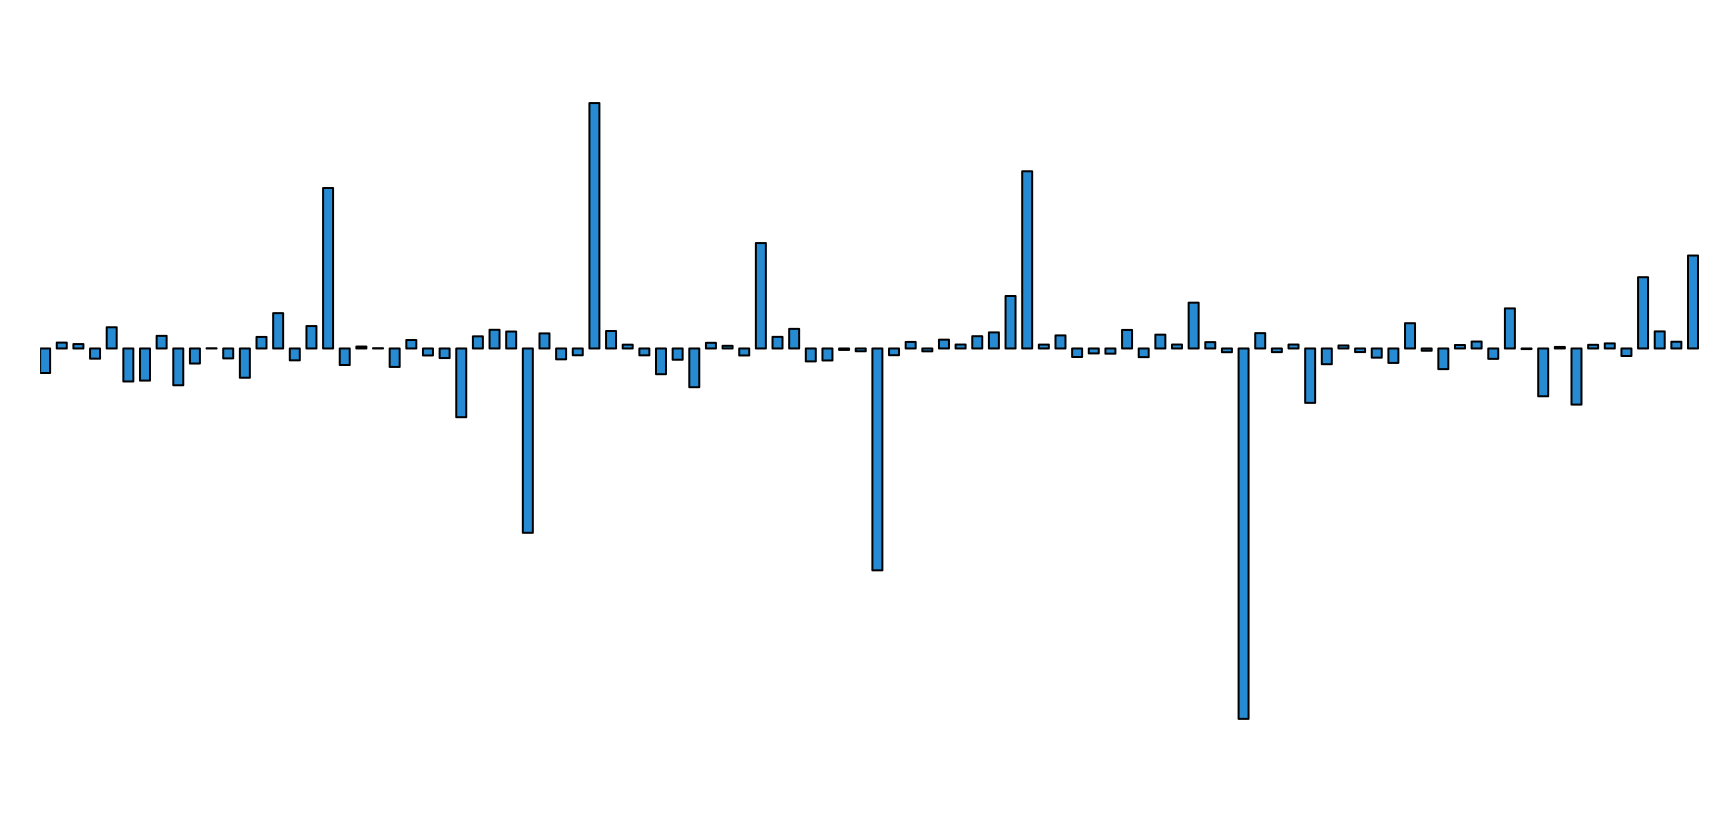
\includegraphics{LevyFlight/levy_length.pdf}
\end{center}
\caption{Distribution de 100 tirages aléatoire obéissant à une distribution de Lévy.
         \label{fig:levy_length}}
\end{figure}

\begin{figure}
\begin{center}
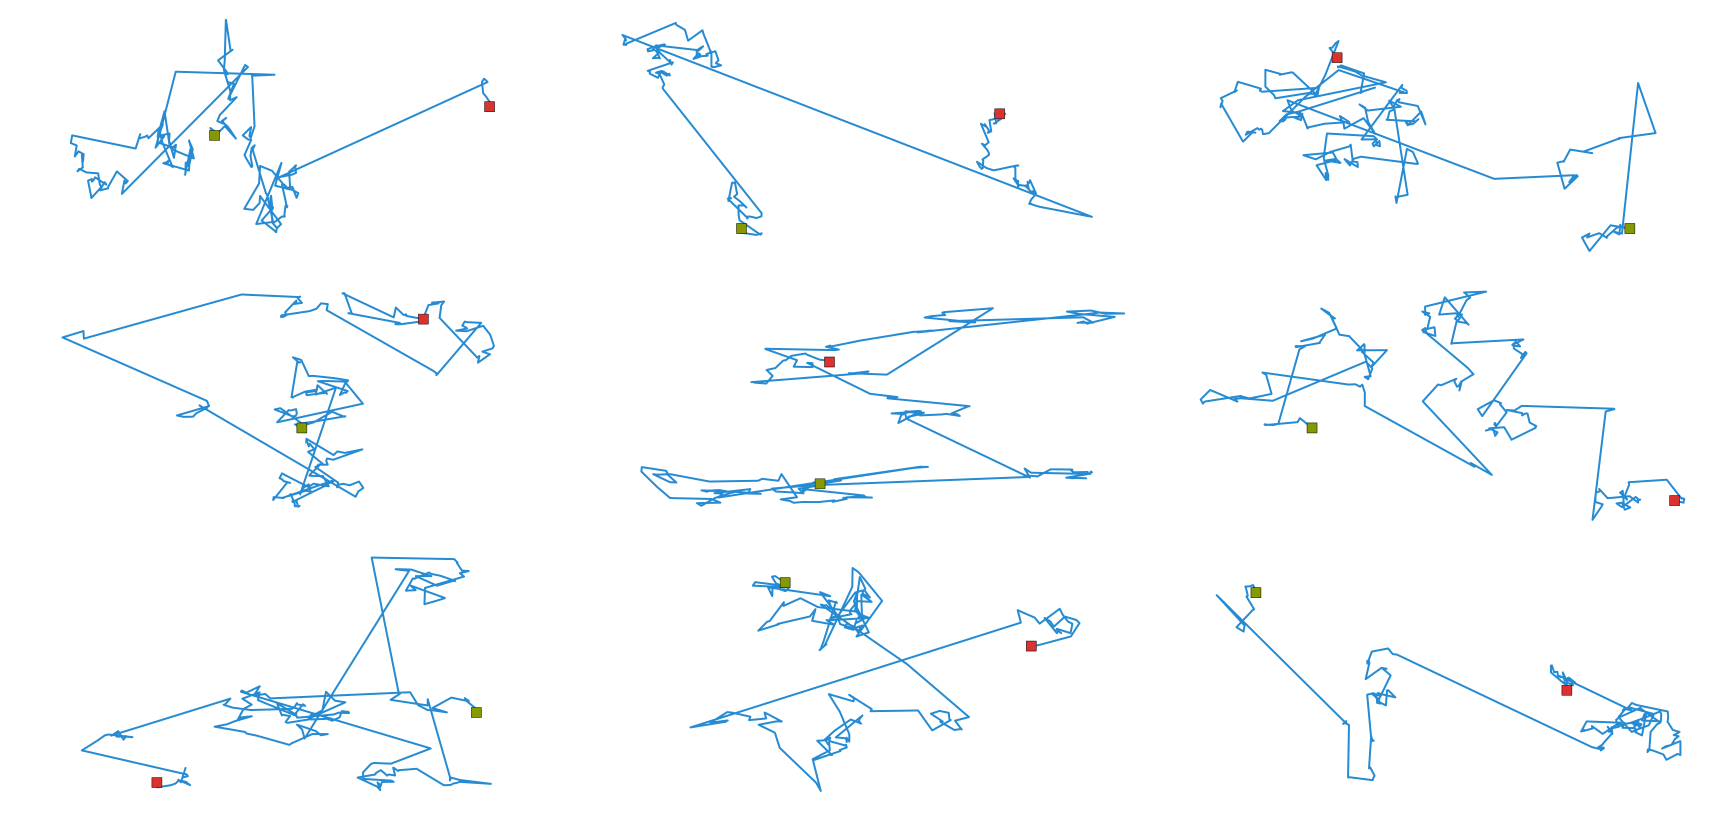
\includegraphics{LevyFlight/levy_flight.pdf}
\end{center}
\caption{Multiple Lévy flight de 200 pas.
         \label{fig:levy_flight}}
\end{figure}

\begin{figure}
\begin{center}
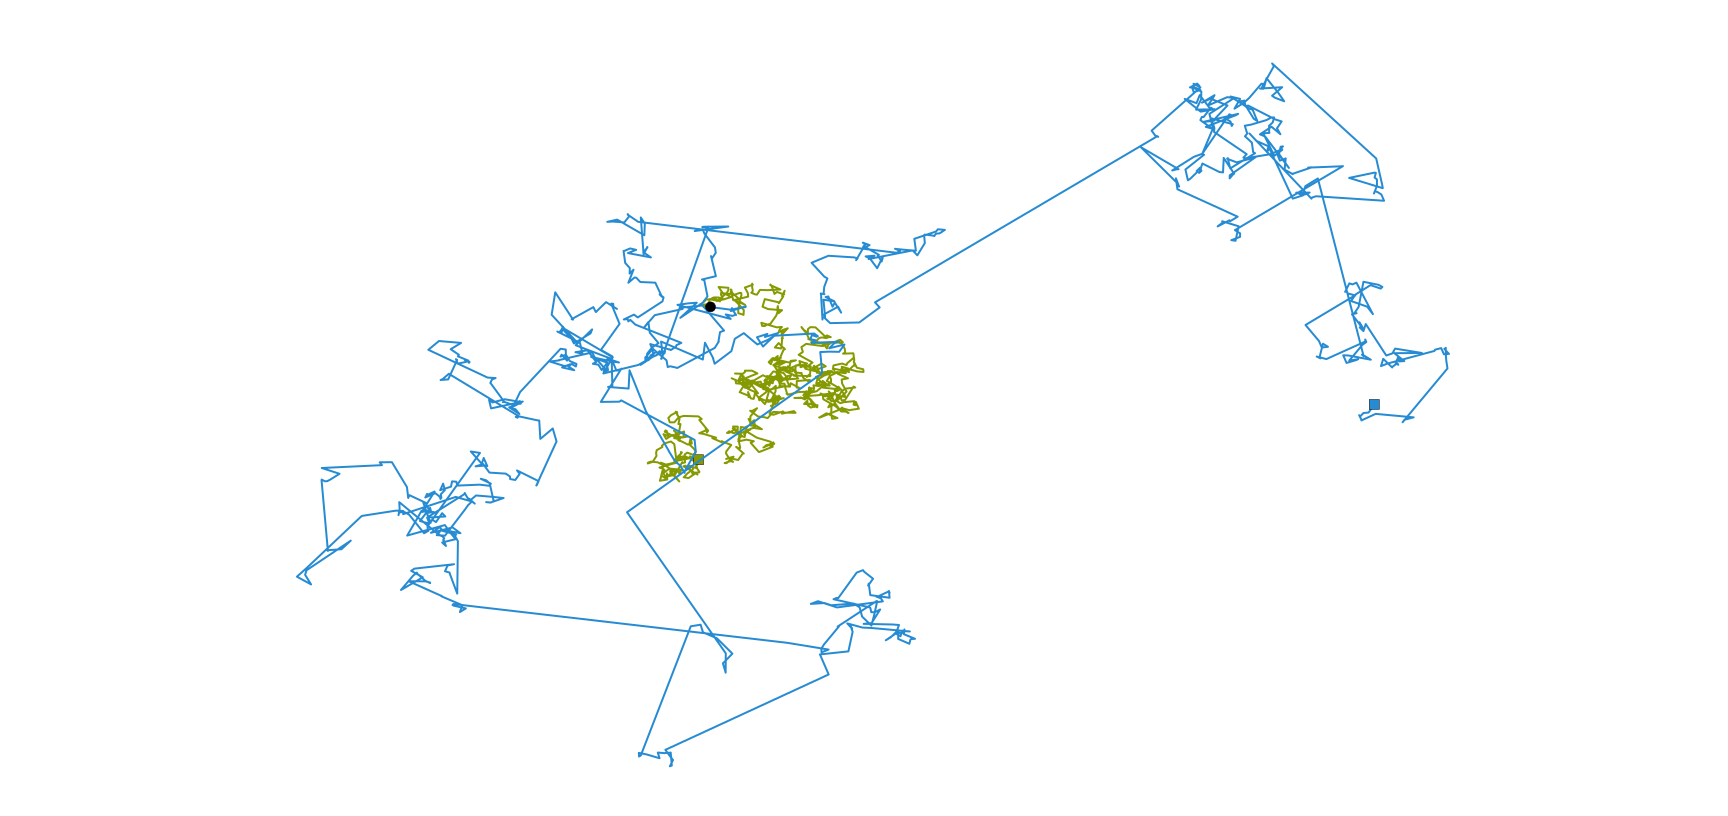
\includegraphics{LevyFlight/levy_vs_gaussian.pdf}
\end{center}
\caption{Mouvement browien (en vert) et Lévy flight (en bleu) pour 200 pas aléatoires.
         \label{fig:levy_vs_gaussian}}
\end{figure}


\itodo{Ajoute des applications aux problèmes multi-critères}
Dans \cite{Sharma2012213}, Lévy flight est employé pour améliorer l’algorithme ABC
pour faire une recherche locale autour de la meilleure solution actuelle. L’auteur
utilise un multiplicateur pour réduire la longueur des pas généré d’après \eqref{eq:step_len}.
De plus la meilleure solution actuelle est utilisée pour guider la recherche aléatoire et
peu être assimilé à un apprentissage.




\ftodo{Le caractère spécifique de cette distribution peut être observé ...}
La distribution traduit le schéma d’une recherche locale suivi par une forte variation. L’utilisation
de cette distribution permet ainsi de renforcer la recherche locale sans prendre le risque de se
coincer dans un optimum local.









\itodo{Décrire apprentissage par opposition et applications.\\
       Ajouter des exemple en multi-objectif pour montrer que c’est applicable}
La recherche par vecteur opposé (opposition-based learning) a été implémenté pour la première fois
en optimisation par \cite{}. Il propose une méthode permettant de diversifier la
population sans connaissances à-priori et ne demandant aucuns paramètres à déterminer.
La méthode est la suivante:
\etodo{Ajouter la formule traduisant le principe de la méthode}


Il est important de noter que les solutions sont comparées deux à deux par tournoi binaire.
Il est ainsi sélectionnée ou la solution initiale ou son opposée.
\ftodo{Illustration du tournoi binaire graphiquement !}

Cette méthode a ensuite été améliorée (\cite{Rahnamayan2008155}) puis adaptée à
l’algorithme Differential evolution (DE). La méthode reprend la définition de base
mais définit plus clairement les limites et la portée de la méthode.
La méthode est utilisée durant la phase d’initialisation pour améliorer la diversité
en générant une population aléatoire de $n$ individus puis $n$ opposées.
Les solutions les plus performantes étant ensuite conservées pour obtenir une population
finale de $n$ individus.
Ensuite durant l’exécution de l’algorithme de nouvelles populations opposées sont générées.
Un coefficient $J_r$ est utilisé pour contrôler la probabilité de générer cette nouvelle
population opposée pour chaque itération.

La méthode a ensuite été testée sur un jeu de 15 fonctions de références (7 uni-modales
et 8 multi-modales). La nouvelle approche permet alors de trouver de meilleurs
résultats sur 14 des 15 fonctions. Il est aussi montré la supériorité de la
sélection par opposition par rapport au caractère aléatoire (\cite{Rahnamayan2008155,Rahnamayan2008906})
\itodo{Ajouter:Les fonctions utilisées ---- Les résultats obtenues}

Ensuite un il est aussi mis en avant que la probabilité de générer une population opposée
doit décroitre au fur et à mesure des itérations. En effet la méthode permet de
réduire l’espace de recherche mais ralenti la convergence une fois cette intervalle
faible. Finalement il est proposé d’utiliser une intervalle pour le coefficient si le problème
ne permet pas de déterminer un nombre fixe d’itération à-priori: $[0.1 < J_r < 0.4]$.

Cette approche a été appliquée avec succès dans le cas de l’algorithme ABC en couplage
avec un opérateur de mutation (\cite{Bi2011174}) ou encore en coopération avec une marche
aléatoire (\cite{Sharma2012213}).

Notre problème ne nous permettant pas d’avoir de connaissance à-priori, il nous est
impossible d’estimer le nombre d’itération nécessaires et l’utilisation d’un coefficient $J_r$
dynamique difficile.
Au vu des recommandations et des applications déjà faites pour des problèmes mono-critères,
ce coefficient sera fixé à 0.1 dans un premier temps.
\ftodo{Ajouter une description graphique de l’approche par vecteur opposé}




\iunsure{Décrire approche par chaos et applications}


\itodo{Décrire certaines approches parallèles (elle ne sont pas parallèle dans le sens que je veux faire)}



\itodo{Inspiration, formalisation, détail des groupes d’abeilles, points forts.}
% subsection optimisation_par_essaim_d_abeilles_un_meta_heuristique_a_population (end)

\subsection{Mise à jour du front de Pareto par epsilon-Dominance} % (fold)
\label{sub:mise_a_jour_du_front_de_pareto_par_epsilon_dominance}
% Description de la mise à jour de l’archive choisie:
%  - Formulation théorique
%  - Graphiquement
\itodo{Décrire la méthode choisie parmis celle détaillées dans le chapitre précédent.}
% subsection mise_a_jour_du_front_de_pareto_par_epsilon_dominance (end)


\subsection{Réduction de la cardinalité par screening} % (fold)
\label{sub:reduction_de_la_cardinalite_par_screening}
% Analyse de sensibilité retenue:
%  - Formulation théorique
%  - Graphiquement
\itodo{Présenter l’analyse de sensibilité choisie ...}
% subsection reduction_de_la_cardinalite_par_screening (end)


\subsection{Processus d’optimisation complet} % (fold)
\label{sub:processus_d_optimisation_complet}
\itodo{Ajouter une vision globale du processus d’optimisation sous forme de graphique
      servant de résumé du chapitre.}
% subsection processus_d_optimisation_complet (end)

